\ylDisplay{Veetünn} % Ülesande nimi
{Mihkel Kree} % Autor
{lõppvoor} % Voor
{2005} % Aasta
{G 5} % Ülesande nr.
{5} % Raskustase
{
% Teema: Vedelike-mehaanika
\ifStatement
Silindriline veetünn, milles hoitakse muutumatut veetaset kõrgusega $h$, on tõstetud horisontaalsele platvormile, mille kõrgus maapinnast on $H$ (vt joonist). Tünni seina kõrgusele $a$ selle põhjast puuritakse auk. Väljuv veejuga puudutab maapinda kaugusel $L$ platvormi jalamist. Graafikul on kujutatud kauguse $L$ sõltuvus augu kõrgusest $x = a/h$. Määrake tünni kõrgus $h$ ning aluse kõrgus $H$ eeldusel, et $h > H$.

\begin{center}
	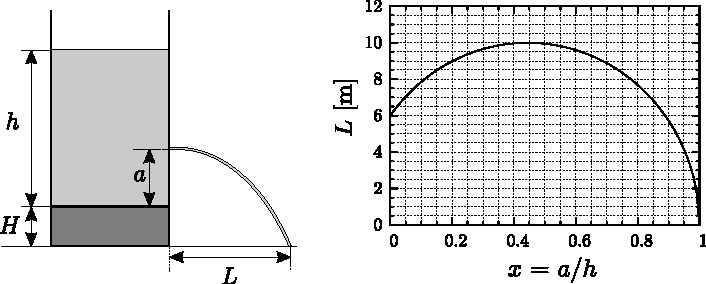
\includegraphics[width=\linewidth]{2005-v3g-05-yl}
\end{center}
\fi


\ifHint
Veejoa väljumise kiirus on leitav energia jäävuse seadusest või alternatiivselt impulsi jäävusest. Mõlemad lähenemised on korrektsed, aga annavad numbrilise konstandi võrra erineva vastuse, mis on tingitud jäävusseaduste kehtivuse eelduste erinevusest. Tünni ja aluse kõrgused on leitavad valides graafikult kaks (või vajadusel rohkem) punkti ja lahendades tekkinud võrrandisüsteemi.
\fi


\ifSolution
Leiame esmalt veejoa väljumise kiiruse. Kiiruse avaldis on tuntud Torricelli seadusena, kuid selle leidmiseks võime arutleda nõnda: avast väljuv juga omab kineetilist energiat $mv^2/2$, teisalt peab see olema võrdne potentsiaalse energiaga, mis saadakse vee ülemiselt pinnalt kuni auguni langedes: $mg(1 - x)h$. Seega väljumiskiirus avaldub kui
\[
v = \sqrt{2g(1 - x)h}.
\]
\emph{Märkus}. impulsi jäävusest saaksime (võrreldes tünni vasakule ja paremale seinale mõjuvate rõhumisjõudude vahe avaldist ning veejoa impulssi) tulemuse $v = \sqrt{g(1 - x)h}$. See avaldis kehtib siis, kui vee liikumine tünnis pole laminaarne ning energia ei säili (läheb veekeeristesse). Laminaarse (energiakadudeta) voolu korral tuleks rõhumisjõudude vahe leidmisel arvestada Bernoulli seadusest tingitud rõhu muutust, mistõttu impulsi jäävusest tuletatud vastus ei kehti. Kuivõrd antud ülesandes on voolu laminaarsuse küsimus jäetud täpsustamata, siis on mõlemad meetodid korrektsed.

Et veejoal vertikaalset kiiruskomponenti esialgu pole, kulub langemiseks aeg
\[
\tau = \sqrt{\frac{2(H+xh)}{g}}.
\]
Selle ajaga liigub aga veejuga horisontaalsihis kaugusele $L = v\tau$ ehk:
\[
L=2 \sqrt{(1-x) h(H+x h)},
\]
mida aga ongi antud graafikul kujutatud.

Seega piisaks $H$ ja $h$ leidmiseks kahe joone punkti koordinaatide määramisest ning tekkiva võrrandisüsteemi lahendamisest. Et aga võimalikult lihtsalt tulemuseni jõuda, kasutame tähelepanekut, et $x = 0$ korral $L = 2\sqrt{hH}$. Võtame graafikult lugemi punktis $x = 0$ ning saame esimese võrrandi: $hH = \SI{9}{m^2}$.

Nagu öeldud, võib teise võrrandi saada suvalise punkti abil, kuid uurime natuke ekstreemumtingimust. Tähistame esmalt $\alpha = H/h$, $L$ avaldub seega kui
\[
L=2 h \sqrt{(1-x)(\alpha+x)}.
\]
Kui võtame $L$-ist $x$-i järgi tuletise, näeme, et $L$ omab ekstreemumväärtust $x = (1 - \alpha )/2$ korral. Selle tulemiseni võib jõuda ka arutledes nõnda: $y = (1-x)(\alpha +x)$ kujutab endast allapoole suunatud parabooli nullkohtadega $1$ ja $-\alpha$, ekstreemumväärtus on seega nende vahel ehk kohal $x = (1 - \alpha )/2$. Asendame selle $L$-i avaldisse:
\[
L=2 h \sqrt{\left(1-\frac{1-\alpha}{2}\right)\left(\alpha+\frac{1-\alpha}{2}\right)}=2 h \frac{1+\alpha}{2}=h+H.
\]
Seega saame teise võrrandi $L$-i maksimumväärtust kasutades:
\[
H + h = \SI{10}{m}.
\]
Nendest kahest lihtsast võrrandist tekkiva võrrandisüsteemi lahendamisel (viies need näiteks ruutvõrrandi kujule) leiame väärtused: $h = \SI{9}{m}$ ja $H = \SI{1}{m}$.
\fi
}